\chapter{Implementación}
\label{ch:implementacion}
Una vez se ha definido en detalle cómo debe ser el sistema, se procede a la implementación de este, de manera que se hagan realidad todas las especificaciones. 

En este capítulo se entra más en detalle en cómo se ha realizado la programación de las distintas partes para que funcionen correctamente y en armonía entre ellas. Se tratarán todas las partes implicadas, desde el servidor en el que se alojan la aplicación y la base de datos, hasta estas mismas y el propio dispositivo que se utiliza para recoger los datos.

\section{Servidor}\label{sec:servidorImpl}
En primer lugar, se debe montar el servidor sobre el que aloja la aplicación y la base de datos, para que de esta manera pueda ser accedido por los usuarios. Como se ha dicho en la \autoref{subsec:servidorDB}, se emplea la herramienta XAMPP para este propósito.

Para comenzar a utilizar XAMPP simplemente se instala el programa en la máquina o servidor que se vaya a utilizar como equipo central. El instalable se puede descargar desde la página oficial~\cite{vmware_xampp_nodate}.

En este caso, en la instalación solo es necesario marcar las opciones de instalar Apache y MySQL, puesto que es suficiente para el funcionamiento de la aplicación.

Cuando se ha instalado, se arranca la herramienta y mediante su interfaz gráfica se pueden configurar los puertos y direcciones sobre las que se quiere que lance Apache y la base de datos MariaDB. Aunque, en la aplicación ponga MySQL se utiliza MariaDB dado que comparten los comandos.

El servidor Apache se lanza sobre el puerto 80 y la base de datos en el puerto 3306, a los que se puede acceder utilizando la IP pública de la máquina o desde la máquina utilizando \textit{localhost}.

\section{Base de datos}\label{sec:base-de-datos}
Cuando se haya lanzado el servidor y hecho clic en \textit{Start} de la base de datos MariaDB, se puede acceder directamente a la interfaz web de phpMyAdmin mediante la dirección \textit{direcciónIP/phpmyadmin}, que permite realizar la configuración completa de la base de datos. En este caso no se ha utilizado la interfaz para configurarlo, sino que se ha utilizado el terminal que ofrece desde la pestaña SQL\@.
\pagebreak

El primer paso es crear en sí la base de datos, donde están las tablas de datos. Para esto se emplea el \autoref{lst:creacionBD}.
\begin{lstlisting}[language=SQL, caption=Creación de la base de datos,label=lst:creacionBD]
CREATE DATABASE tfg_db;
\end{lstlisting}

A continuación se crea un usuario con todos los permisos, que es el que emplea el administrador de la base de datos y que le permite añadir las credenciales de acceso de los usuarios a la aplicación. Por otro lado, se tiene otro usuario con permisos de inserción y actualización de registros, que es el utilizado por el dispositivo, dado que este añade medidas y actualiza su estado. Para lograr esto se introduce el \autoref{lst:creacionUsuarios}.
\begin{lstlisting}[language=SQL, caption=Creación de usuarios de la base de datos, label=lst:creacionUsuarios]
CREATE USER 'tfg_user'@'%' IDENTIFIED BY 'tfg_pass';
GRANT ALL PRIVILEGES ON tfg_db.* TO 'tfg_user'@'%';
CREATE USER 'device_user'@'%' IDENTIFIED BY 'device_pass';
GRANT SELECT, INSERT, UPDATE ON *.* TO 'device_user'@'%';
\end{lstlisting}

Una vez se han creado los accesos, se procede a elaborar las tablas que se utilizan en la aplicación, que son: la de medidas (\textit{sensor\_data}), la de dispositivos (\textit{devices}) y la de usuarios (\textit{users}). Están formadas por los campos y relaciones descritas en la \autoref{sec:modelo} y los comandos correspondientes para su creación son el \autoref{lst:creacionTablas}.
\begin{lstlisting}[language=SQL, caption=Creación de tablas de la base de datos, label=lst:creacionTablas]
CREATE TABLE sensor_data (
    date datetime NOT NULL,
    device varchar(50) NOT NULL,
    temperature float NOT NULL,
    humidity float NOT NULL,
    pm2_5 float NOT NULL,
    pm10 float NOT NULL,
    co float NOT NULL,
    co2 mediumint(9) NOT NULL,
    PRIMARY KEY (date, device),
    CONSTRAINT deviceData FOREIGN KEY (device) 
    REFERENCES devices(id) ON DELETE CASCADE ON UPDATE CASCADE
);

CREATE TABLE devices (
    id varchar(50) NOT NULL,
    ip varchar(16) NOT NULL,
    date varchar(19) NOT NULL,
    status varchar(7) NOT NULL,
    PRIMARY KEY (id)
);

CREATE TABLE users (
    username varchar(32) NOT NULL,
    password varchar(32) NOT NULL,
    PRIMARY KEY (username)
);
\end{lstlisting}

Por parte de la base de datos este es el proceso que hay que realizar, pero en la \autoref{sec:implAplicacion} se explica cómo se realizan las consultas y en la \autoref{sec:implDispositivo} como se ejecutan las inserciones y actualizaciones.

\section{Aplicación web}\label{sec:implAplicacion}
En esta sección se explica cómo se ha implementado la lógica de las páginas vistas en la \autoref{sec:interfaz}, así como la definición de la estructura que las forman. Como se especificó en la \autoref{subsec:lenguajes} la página se ha implementado en HTML, CSS y PHP en el entorno de Visual Studio Code.

\subsection{Página: Inicio de sesión}\label{subsec:página-inicio-de-sesión}
Esta primera pantalla comprueba primero si la sesión esta iniciada, si es así se redirige a la página principal. Por el contrario, si no está iniciada aparece un formulario de HTML en el que se solicita el usuario y contraseña. 

En este formulario, al hacer \textit{submit} (botón "<Iniciar sesión">) se activa un script que comprueba si los campos han sido rellenados o no, de manera que salte un \textit{alert} avisando al usuario. Si los campos están rellenos, se pasa a comprobar si el usuario existe en la base de datos, para lo que, en primer lugar, se pasa la contraseña a MD5 por seguridad y después se realiza una consulta a la tabla de \textit{users} de la base de datos. Si la consulta tiene éxito se crea una sesión y se redirige a la página principal, de lo contrario se muestra un \textit{alert} avisando al usuario de que no existe como tal y que revise las credenciales.

La lógica explicada se ha extraído de \textit{Webslesson}~\cite{webslesson_php_nodate} y se ha modificado para adaptarla a la aplicación, quedando el \autoref{lst:comprobacionFormularioInicioSesion}.
\begin{lstlisting}[language=PHP, caption=Comprobación formulario Inicio de sesión, label=lst:comprobacionFormularioInicioSesion]
$connect = mysqli_connect("localhost", "tfg_user", "tfg_pass", "tfg_db");
session_start();
if (isset($_SESSION["username"])) {
    header("location:main.php");
}
if (isset($_POST["login"])) {
    if (empty($_POST["username"]) && empty($_POST["password"])) {
        echo '<script>alert("Ambos campos son obligatorios")</script>';
    } else {
        $username = mysqli_real_escape_string($connect, $_POST["username"]);
        $password = mysqli_real_escape_string($connect, $_POST["password"]);
        $password = md5($password);
        $query = "SELECT * FROM users WHERE username = '$username' AND password = '$password'";
        $result = mysqli_query($connect, $query);
        if (mysqli_num_rows($result) > 0) {
            $_SESSION['username'] = $username;
            header("location:main.php");
        } else {
            echo '<script>alert("Compruebe las credenciales")</script>';
        }
    }
}
\end{lstlisting}

En el caso de que se cierre la sesión, se elimina la sesión y se redirige al usuario a esta página, para esto se pasa primero a una página temporal llamada \textit{logout.php} que tiene el \autoref{lst:borradoSesion}.
\begin{lstlisting}[language=PHP, caption=Borrado de sesión y redirección a la página de inicio, label=lst:borradoSesion]
session_start();
session_destroy();
header("location:index.php?action=login");
\end{lstlisting}

\subsection{Página: Principal}\label{subsec:implPagPrincipal}
Es la página a la que se accede una vez se inicia la sesión, por lo que lo primero que se comprueba es que haya una sesión de usuario iniciada, si no lo está, se redirige a la página de inicio de sesión siguiendo el \autoref{lst:redireccionInicioSesion}.
\begin{lstlisting}[language=PHP, caption=Redirección a la página de inicio de sesión si sesión no iniciada, label=lst:redireccionInicioSesion]
session_start();
if (!isset($_SESSION["username"])) {
    header("location:index.php?action=login");
}
\end{lstlisting}

El contenido que se muestra se genera de manera dinámica, de forma que el saludo del título es el nombre de usuario de la sesión iniciada. Esto se hace con el \autoref{lst:saludoPagPrincipal}.
\pagebreak

\begin{lstlisting}[language=PHP, caption=Saludo página principal, label=lst:saludoPagPrincipal]
echo '<h1>Bienvenido, ' . $_SESSION["username"] . '</h1>';
\end{lstlisting}

Por otro lado, para generar la tabla es necesario previamente conectar con la base de datos. Una vez se establece la conexión con éxito, lo que se hace es consultar la tabla de \textit{devices} para obtener los dispositivos que están registrados en la aplicación y su estado, y por cada uno de los registros se genera una fila de la tabla. La tabla completa se genera con el siguiente fragmento de \autoref{lst:tablaDispositivos}.
\begin{lstlisting}[language=PHP, caption=Visualización de tabla de dispositivos, label=lst:tablaDispositivos]
$connect = mysqli_connect("localhost", "tfg_user", "tfg_pass", "tfg_db");

$query = "SELECT * FROM devices";
$result = mysqli_query($connect, $query);
echo "<table class='tables'>
<tr>
    <th>Nombre del dispositivo</th>
    <th>Estado</th>
    <th>Ultimo cambio de estado</th>
    <th>Control</th>
</tr>";

while ($row = mysqli_fetch_array($result)) {
    echo "<tr>";
    echo "<td>" . $row['id'] . "</td>";
    echo "<td>" . $row['status'] . "</td>";
    echo "<td>" . $row['date'] . "</td>";
    echo '<td><button class="boton" onclick="location.href=\'device.php?id=' . $row['id'] . '&ip=' . $row['ip'] . '\'">Acceder</button></td>';

    echo "</tr>";
}
echo "</table>";
\end{lstlisting}

Como se puede ver en la última columna de cada fila, hay un botón cuya acción es redirigir a la página del propio dispositivo, pasando como parámetros el id del dispositivo y la IP de este.

Por último, el botón de cerrar sesión lleva a la página \textit{logout.php} que se describe al final de la \autoref{subsec:implPagPrincipal}.

\subsection{Página: Dispositivo}\label{subsec:página-dispositivo}
Como se hace en las demás páginas, en primer lugar se comprueba si la sesión esta iniciada, si no lo está, se redirige a la página de inicio de sesión.

Esta página es similar a la de la \autoref{subsec:implPagPrincipal} en cuanto a que, lo primero que hace es mostrar el nombre del dispositivo como ocurre con el saludo, pero en este caso se extrae de la URL\@.
\begin{lstlisting}[language=PHP, caption=Nombre del dispositivo en la cabecera de la página, label=lst:nombreDispositivo]
echo '<h1>' . $_GET["id"] . '</h1>';
\end{lstlisting}

Para mostrar la imagen en tiempo real de dicho dispositivo, se utiliza un elemento \textit{img}, en el que se vuelca la imagen que está transmitiendo el dispositivo sobre el puerto 8000 de su dirección IP obtenida del URL, que se corresponde con la línea de \autoref{lst:imgCamara}.
\begin{lstlisting}[language=PHP, caption=Cuadro de imagen de la cámara, label=lst:imgCamara]
echo '<img src="http://' . $_GET["ip"] . ':8000/stream.mjpg" id="cam">'
\end{lstlisting}

En cuanto a las gráficas, se emplea una librería de Google llamada \textit{Google Charts} que permite definir gráficas a partir de los datos extraídos mediante una consulta a base de datos. En este caso, las medidas que se emplean son las que corresponden al dispositivo de la página. Para emplear esta librería se debe definir una función que escriba sobre elementos \textit{div} las gráficas, en este caso se hace mediante la función \textit{drawChart()} que se define según el \autoref{lst:graficasDispositivo}.
\begin{lstlisting}[language=PHP, caption=Gráficas de las medidas del dispositivo, label=lst:graficasDispositivo]
$chartQuery = 'SELECT * FROM (SELECT * FROM sensor_data WHERE device="' . $_GET["id"] . '" ORDER BY date DESC LIMIT 720) sub ORDER BY date ASC';
$chartQueryRecords = mysqli_query($con, $chartQuery);

function drawCharts() {
    var data = google.visualization.arrayToDataTable([
        ['Fecha', 'Temperatura', 'Humedad', 'PM2.5', 'PM10', 'CO', 'CO2'],
        <?php
        while ($row = mysqli_fetch_assoc($chartQueryRecords)) {
            echo "['" . $row['date'] . "'," . $row['temperature'] . "," . $row['humidity'] . "," . $row['pm2_5'] . "," . $row['pm10'] . "," . $row['co'] . "," . $row['co2'] . "],";
        }
        ?>
    ]);
    var options = {
        legend: {
            position: 'top',
            alignment: 'start'
        }
    };

    var view = new google.visualization.DataView(data);
    view.setColumns([0, 1, 2]);
    var view2 = new google.visualization.DataView(data);
    view2.setColumns([0, 3, 4, 5]);
    var view3 = new google.visualization.DataView(data);
    view3.setColumns([0, 6]);

    var chart = new google.visualization.LineChart(document.getElementById('regions_temp_hum'));
    chart.draw(view, options);
    var chart = new google.visualization.LineChart(document.getElementById('regions_pm_co'));
    chart.draw(view2, options);
    var chart = new google.visualization.LineChart(document.getElementById('regions_co2'));
    chart.draw(view3, options);
}
<div id="regions_temp_hum" class="grafica"></div>
<div id="regions_pm_co" class="grafica"></div>
<div id="regions_co2" class="grafica"></div>
\end{lstlisting}

Se puede ver que se define una única gráfica con todas las medidas en función del tiempo. Estas medidas se obtienen mediante una consulta a la tabla \textit{sensor\_data} de la que se obtienen 720 registros ordenados por fecha descendente. Esta gráfica grande se parte más tarde en 3 gráficas más pequeñas, indicando qué columnas se quiere que aparezcan en cada una de ellas. En último lugar, se indica que sean de tipo gráfico de línea y que se muestren en los elementos con el id \textit{regions\_temp\_hum}, \textit{regions\_pm\_co} y \textit{regions\_co2}.

Dado que la página con todos los elementos se vuelve muy larga, se ha añadido en varios puntos un botón "<Volver"> que redirige a la página principal.
\begin{lstlisting}[language=HTML, caption=Botón de retorno a página principal, label=lst:botonVolver]
<button class="boton" id="boton_volver" onclick="location.href=' main.php'">Volver</button>
\end{lstlisting}

Al final, para mostrar la tabla de medidas se hace una consulta a la tabla \textit{sensor\_data} de la que se obtienen los últimos 500 registros ordenados de más reciente a más antiguo del dispositivo correspondiente, estas medidas se introducen de manera dinámica como filas con el \autoref{lst:tablaMedidas}.
\begin{lstlisting}[language=PHP, caption=Visualización tabular de las medidas del dispositivo, label=lst:tablaMedidas]
$query = 'SELECT * FROM sensor_data WHERE device="' . $_GET["id"] . '" ORDER BY date DESC LIMIT 500';
$result = mysqli_query($con, $query);
echo "<table class='tables'>
<tr>
    <th>Fecha</th>
    <th>Temperatura</th>
    <th>Humedad</th>
    <th>PM<sub>2.5</sub></th>
    <th>PM<sub>10</sub></th>
    <th>CO</th>
    <th>CO<sub>2</sub></th>
</tr>";
while ($row = mysqli_fetch_array($result)) {
    echo "<tr>";
    echo "<td>" . $row['date'] . "</td>";
    echo "<td>" . $row['temperature'] . "</td>";
    echo "<td>" . $row['humidity'] . "</td>";
    echo "<td>" . $row['pm2_5'] . "</td>";
    echo "<td>" . $row['pm10'] . "</td>";
    echo "<td>" . $row['co'] . "</td>";
    echo "<td>" . $row['co2'] . "</td>";
    echo "</tr>";
}
echo "</table>";
\end{lstlisting}

\section{Dispositivo}\label{sec:implDispositivo}
La base del dispositivo es una Raspberry Pi 3B+ con las características detalladas en la \autoref{subsec:altPlacas} y con el sistema operativo Raspbian, que proporciona un entorno similar a Linux sobre el que empezar a trabajar.

En primer lugar, se conectan los sensores y la cámara a los puertos que se han explicado en la \autoref{sec:hardware}, de manera que la distribución de los elementos del dispositivo es la mostrada en la \autoref{fig:circuito}. Cuando ya está todo montado correctamente, se puede pasar a conectarlo a la red y a la corriente eléctrica para comenzar con su configuración.

En cuanto a las configuraciones previas, primero se habilita el puerto CSI para la cámara a través de \textit{raspi-config}, después, dado que se emplea un puerto USB para el sensor de partículas en suspensión se utiliza \textit{dmesg} para identificar cuál es la interfaz usada. Cuando el programa ya está completo se añade como proceso que se ejecuta al iniciar el sistema, de esta manera solo hace falta configurarlo una vez y conectarlo en el lugar donde se desee utilizar.
\pagebreak

Una vez realizada esta configuración se pasa a desarrollar el programa en el lenguaje Python utilizando como entorno de desarrollo PyCharm, con el que mediante SSH se conecta a la Raspberry Pi, lo que se especifica previamente en la \autoref{subsec:lenguajes}.

En las siguientes subsecciones se explican cada una de las clases que componen el programa y en la última el programa principal que las relaciona a todas ellas.

\subsection{Clase de la Cámara}\label{subsec:clase-de-la-cámara}
El objetivo de esta clase es ofrecer al programa principal, mediante una función, la facilidad de transmitir vía IP la imagen en tiempo real que capta la cámara instalada en el puerto CSI. Para el desarrollo de esta función se ha consultado el artículo \textit{How to Set Up Real-Time Video Using OpenCV on Raspberry Pi 4}~\cite{addison_how_nodate} en el que se explica de manera detallada como poner a punto la Raspberry y acceder al puerto CSI de esta.

Se ha empleado la librería \textit{picamera}~\cite{jones_picamera_nodate} para acceder a la imagen de la cámara, para lo que se utiliza una resolución de 640x480 píxeles a una tasa de refresco de 24 fotogramas, suficiente para ver con claridad el interior de la sala y que no consuma mucha energía.

En cuanto a la retransmisión de la imagen se lanza un servidor local montado en el puerto 8000 mediante \textit{http.server}, sobre el que se vuelca el vídeo y de esta manera se muestra en la web.

El vídeo comienza a transmitirse de manera inmediata y cuando el programa lance una excepción de finalización se cierra.

\subsection{Clase del sensor CO}\label{subsec:clase-del-sensor-co}
Como se menciona en la \autoref{sec:hardware} el sensor de CO es analógico, por lo que en primer lugar hay que vincular los puertos de la Raspberry para que mande las señales correspondientes al conversor MCP3008, y una vez interpretadas las devuelva a la Raspberry. Esta asignación se basa en los \textit{drivers} de osoyoo~\cite{osoyoo_osoyoodriver_2021}, pero adaptada a los puertos de este proyecto.

El código de este sensor se encarga fundamentalmente de realizar la lectura de la señal del conversor y convertir el voltaje recibido a porcentaje de monóxido de carbono en el ambiente, esto se calcula con $\frac{\textit{Voltaje}\cdot 100}{1024}$.

Antes de empezar a realizar mediciones necesita un tiempo de calentamiento de 20 segundos, a partir de este punto es capaz de hacer mediciones de manera continua.

\subsection{Clase del sensor \texorpdfstring{CO$_2$}{CO2}}\label{subsec:clase-del-sensor-co2}
Para obtener las partes por millón de dióxido de carbono del ambiente se sigue el proceso que describe el manual del sensor MH-Z14~\cite{zhengzhou_winsen_electronics_technology_users_nodate}, que se puede ver en la \autoref{fig:co2PPMcalc}.
\begin{figure}[H]
	\ffigbox[\textwidth]
	{\caption{Lectura de concentración de CO$_2$ MH-Z14}
		\label{fig:co2PPMcalc}}
	{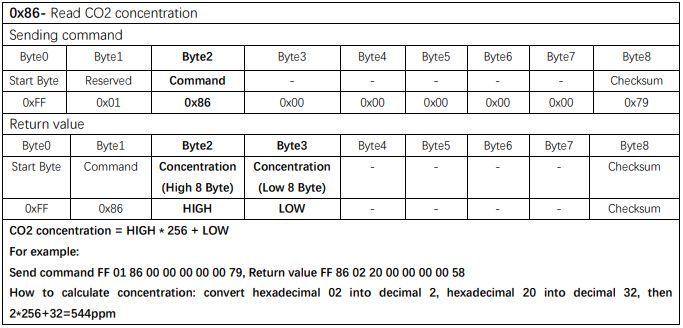
\includegraphics[width=\textwidth]{co2ppm.jpg}}
\end{figure}
En primer lugar hay que identificar en qué puerto serial se encuentra el sensor, en este caso es el \textit{ttyS0} que corresponde al puerto UART. Tras esto, simplemente se realiza una \textit{request} de lectura que se indica en la \autoref{fig:co2PPMcalc} y de la que se obtiene como respuesta el valor de la concentración de CO$_2$ junto con un \textit{checksum} para verificar que la lectura es correcta.

La función principal de esta clase es el método \textit{get()} que devuelve el número de partes por millón, este valor se calcula con el \autoref{lst:co2PPMcalc}, que es una simplificación de esta clase.
\begin{lstlisting}[language=Python, label=lst:co2PPMcalc, caption=Cálculo de la concentración de CO$_2$]
serial = serial.Serial(port='/dev/ttyS0', timeout=1)
request = [0xff, 0x01, 0x86, 0x00, 0x00, 0x00, 0x00, 0x00, 0x79]
serial.write(bytearray(request))
response = serial.read(9)
return (response[2] << 8) | response[3]
\end{lstlisting}

\subsection{Clase del sensor Temperatura y Humedad}\label{subsec:clase-del-sensor-temperatura-y-humedad}
Esta clase consta de un único método, \textit{tempHumSensor()}, que devuelve la temperatura y la humedad del ambiente en una dupla (temperatura, humedad). Para conseguir esto se utiliza la librería \textit{Adafruit\_DHT}~\cite{adafruit_dht_nodate} que es específica de este tipo de sensores de temperatura y humedad.

Primero se crea un objeto del tipo específico del sensor, en este caso DHT11, y una variable que indica el puerto GPIO al que está conectado el sensor. Con estos dos elementos ahora se pueden hacer lecturas. Estas llamadas devuelven la dupla (temperatura, humedad) que tras realizar una serie de comprobaciones de valores nulos o atípicos es la salida del método. En el \autoref{lst:tempHumSensor} se puede contemplar esta lógica.
\begin{lstlisting}[language=Python, label=lst:tempHumSensor, caption=Lectura de la temperatura y humedad]
def tempHumSensor(self):
    dht_sensor = Adafruit_DHT.DHT11
    dht_pin = 4

    new_humidity, new_temperature = Adafruit_DHT.read(dht_sensor, dht_pin)
    if (new_humidity is None and new_temperature is None) or new_temperature not in range(0, 101) or \
            new_humidity not in range(0, 101):
        if (self.humidity is None and self.temperature is None) or self.temperature not in range(0, 101) or \
                self.humidity not in range(0, 101):
            while (new_humidity is None and new_temperature is None) or new_temperature not in range(0, 101) or \
                    new_humidity not in range(0, 101):
                new_humidity, new_temperature = Adafruit_DHT.read(dht_sensor, dht_pin)
                self.humidity, self.temperature = new_humidity, new_temperature
        return self.temperature, self.humidity
    else:
        self.humidity, self.temperature = new_humidity, new_temperature
        return self.temperature, self.humidity
\end{lstlisting}

\subsection{Clase de la Base de datos}\label{subsec:clase-de-la-base-de-datos}
En primer lugar, el constructor de esta clase se encarga de establecer la conexión con la base de datos, en este caso se utiliza la librería \textit{mysql.connector} y el método \textit{connect(host, user, password, database)}, cuyos parámetros se reciben al instanciar el objeto. Se puede ver en el \autoref{lst:cdb} el fragmento correspondiente.
\begin{lstlisting}[language=Python, label=lst:cdb, caption=Conexión con la base de datos]
def __init__(self, host, user, password, database):
    self.mydb = mysql.connector.connect(
        host=host,
        user=user,
        password=password,
        database=database,
    )
\end{lstlisting}

En cuanto a los métodos que lo componen hay dos, uno para registrar mediciones y otro para registrar el estado del dispositivo. Para la inserción de las mediciones se construye una solicitud de \textit{INSERT} a la tabla \textit{sensor\_data} con todas las medidas recibidas en forma de JSON, después se ejecuta la consulta y si tiene éxito continuamos. Este método se puede ver en el \autoref{lst:medidasDB}, al final del cual se imprime por pantalla una confirmación de los datos registrados.
\begin{lstlisting}[language=Python, label=lst:medidasDB, caption=Inserción de mediciones en la base de datos]
def insert_sensor_data_DB(self, values):
    with self.mydb.cursor() as mycursor:
        sql = "INSERT INTO sensor_data (date, device, temperature, humidity, pm2_5, pm10, co, co2)" \
                "VALUES (%s, %s, %s, %s, %s, %s, %s, %s); "
        val = (
            values["date"],
            values["device"],
            values["temperature"],
            values["humidity"],
            values["pm2_5"],
            values["pm10"],
            values["co"],
            values["co2"],
        )
        mycursor.execute(sql, val)
        self.mydb.commit()
        print(val, "inserted.")
\end{lstlisting}

En el otro método se trata de introducir en la tabla \textit{devices} el estado del dispositivo que se recibe en formato JSON. Si el dispositivo no está registrado se completa con éxito el \textit{INSERT} y termina, pero si no es así, se produce un error de inserción y se pasa a hacer un \textit{UPDATE} del registro del dispositivo correspondiente. Como en el método anterior se imprime por pantalla la consulta ejecutada, en el \autoref{lst:estadoDB} se aprecia cómo se hace.
\begin{lstlisting}[language=Python, label=lst:estadoDB, caption=Inserción de estado del dispositivo en la base de datos]
def insert_update_device_DB(self, params):
    with self.mydb.cursor() as mycursor:
        sql = "INSERT INTO devices (id, ip, date, status) VALUES (%s, %s, %s, %s)"
        val = (
            params["device"],
            params["ip"],
            params["date"],
            params["status"],
        )
        try:
            mycursor.execute(sql, val)
            self.mydb.commit()
            print(params["device"], "inserted")
        except mysql.connector.errors.IntegrityError:
            sql = "UPDATE devices SET date=%s, ip=%s, status=%s WHERE id=%s"
            val = (params["date"], params["ip"], params["status"], params["device"])
            mycursor.execute(sql, val)
            self.mydb.commit()
            print(params["device"], "updated to", params["status"])
\end{lstlisting}

\subsection{Programa Principal}\label{subsec:programa-principal}
En esta última subsección se encuentra el programa que reúne todas las clases descritas anteriormente, cuya función es proporcionar un método sencillo de ejecutar la funcionalidad completa del dispositivo de control ambiental y videovigilancia.

Para empezar, se importan todas las clases descritas y se define el constructor de la clase \textit{cpdDevice}, que es la propia de este programa, en el cual se hace \textit{start()} para iniciar el programa.

El método principal, \textit{start()}, como se ha dicho, inicia el programa y esto requiere los siguientes pasos:
\begin{enumerate}
	\item Iniciar la conexión con la base de datos e introducir/actualizar el estado del dispositivo, que lo pasa a estado \textit{Online}.
	\item Empezar la transmisión de la cámara.
	\item Instanciar los sensores de temperatura y humedad, partículas en suspensión, CO y CO$_2$. Para el de partículas en suspensión, SDS011, se ha utilizado la librería \textit{RPi\_Air\_Quality\_Sensor}~\cite{rovai_python4ds_2021} que mediante una llamada \textit{query()} devuelve las dos medidas necesarias.
	\item Se produce una pausa para el calentamiento de los sensores de 20 segundos.
	\item En bucle, cada 5 segundos, se realiza la lectura de las medidas de temperatura y humedad, partículas en suspensión, CO y CO$_2$ y se registran en la base de datos, junto con la fecha e id del dispositivo.
	\item En caso de interrupción se limpia la asignación de los puertos GPIO, se apaga el sensor de partículas en suspensión y se manda la última actualización de estado indicando que se pasa a estado \textit{Offline}.
\end{enumerate}

El método \textit{start()} es el mostrado en el \autoref{lst:metodoPrincipal}, en el que se recogen todos los pasos descritos.
\pagebreak

\begin{lstlisting}[language=Python, label=lst:metodoPrincipal, caption=Método start del programa principal]
try:
    print("Sensors warming up...")
    # Start dust sensor
    dust_sensor.sleep(sleep=False)

    # Start CO sensor
    co_sensor = COSensor()
    time.sleep(15)

    while True:
        time.sleep(5)

        temperature, humidity = temp_hum_sensor.tempHumSensor()
        co = co_sensor.co_sensor_readadc()
        co2 = co2_sensor.get()
        pm2_5, pm10 = dust_sensor.query()

        # Insert measurements
        data = {
            "date": datetime.now().strftime("%Y-%m-%d %H:%M:%S"),
            "device": self.get_device_id(),
            "temperature": temperature,
            "humidity": humidity,
            "pm2_5": pm2_5,
            "pm10": pm10,
            "co": str("%.2f" % ((co / 1024.) * 100)),
            "co2": co2,
        }
        db.insert_sensor_data_DB(data)

except KeyboardInterrupt:
    GPIO.cleanup()

    # Stop dust sensor
    dust_sensor.sleep(sleep=True)

    # Update device to Offline
    device_params = {
        "date": datetime.now().strftime("%Y-%m-%d %H:%M:%S"),
        "ip": self.get_ip(),
        "status": "Offline",
        "device": self.get_device_id(),
    }
    db.insert_update_device_DB(device_params)
\end{lstlisting}
\pagebreak

Además, se utilizan dos métodos auxiliares, \textit{get\_device\_id()} y \textit{get\_ip()}.  

El \textit{get\_device\_id()} se utiliza para obtener el id del dispositivo, que se corresponde con su dirección física (MAC), para esto se hace uso de la librería \textit{uuid}. Se corresponde con el \autoref{lst:getDeviceId}.
\begin{lstlisting}[language=Python, label=lst:getDeviceId, caption=Método get\_device\_id()]
def get_device_id(self):
    return ':'.join(['{:02x}'.format((uuid.getnode() >> ele) & 0xff) for ele in range(0, 8 * 6, 8)][::-1])
\end{lstlisting}

El \textit{get\_ip()} devuelve la dirección IP del dispositivo, que se obtiene gracias a una llamada de \textit{connect} de la librería \textit{socket}. Este valor se utiliza para retransmitir el vídeo de la cámara y forma parte del registro de estado de la tabla \textit{devices}. En caso de que no se produzca conexión se devuelve una por defecto. En el fragmento de \autoref{lst:getIp} se puede contemplar este proceso.
\begin{lstlisting}[language=Python, label=lst:getIp,caption=Método get\_ip()]
def get_ip(self):
    s = socket.socket(socket.AF_INET, socket.SOCK_DGRAM)
    try:
        s.connect(('10.255.255.255', 1))
        ip = s.getsockname()[0]
    except Exception:
        ip = '127.0.0.1'
    finally:
        s.close()
    return ip
\end{lstlisting}